{
\newcommand{\figWidtha}{7cm}
\newcommand{\trimfiga}[2]{\trimPlotb{#1}{#2}{.02}{.2}{.05}{.1}}
% \newcommand{\figWidth}{5.5cm}
% \newcommand{\clipfig}[2]{\clipFig{#1}{#2}{.02}{.80}{.05}{.90}}
%\newcommand{\cbWidth}{6.0cm}
%\newcommand{\clipfigcb}[2]{\clipFig{#1}{#2}{.881}{.918}{.118}{.885}}
\begin{figure}[hbt]
\begin{center}
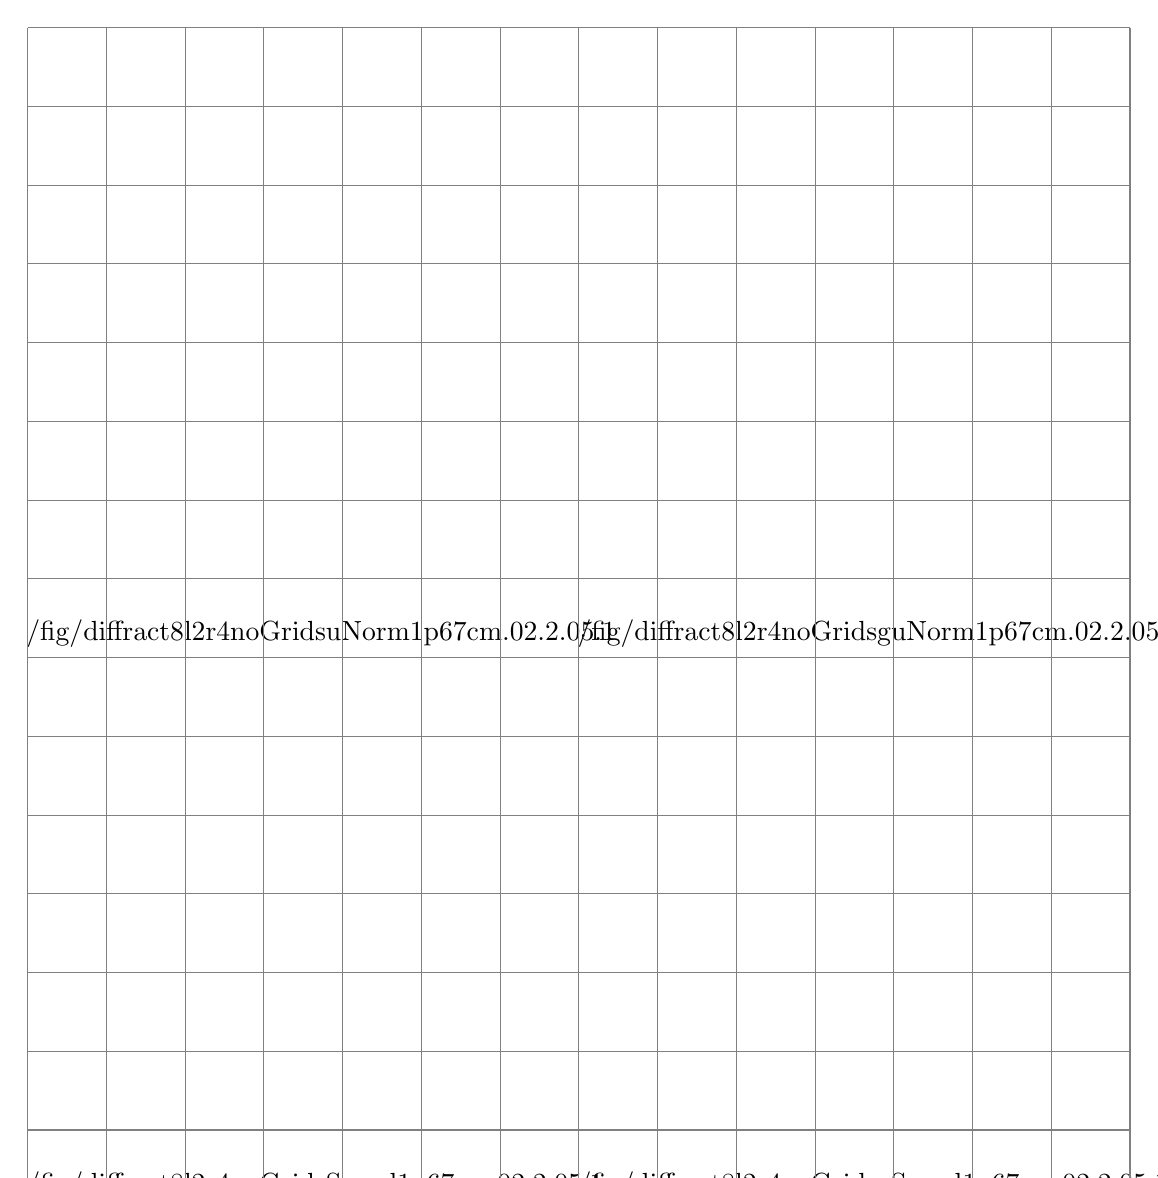
\begin{tikzpicture}[scale=1]
  \useasboundingbox (0,.75) rectangle (14.0,15.);  % set the bounding box (so we have less surrounding white spa  
  \draw ( 0.0,7.0) node[anchor=south west,xshift=-4pt,yshift=+0pt] {\trimfiga{\smDocDir/fig/diffract8l2r4noGridsuNorm1p6}{\figWidtha}};
  \draw ( 7.0,7.0) node[anchor=south west,xshift=-4pt,yshift=+0pt] {\trimfiga{\smDocDir/fig/diffract8l2r4noGridsguNorm1p6}{\figWidtha}};
  \draw ( 0.0,0.0) node[anchor=south west,xshift=-4pt,yshift=+0pt] {\trimfiga{\smDocDir/fig/diffract8l2r4noGridsSpeed1p6}{\figWidtha}};
  \draw (7.0,0.0) node[anchor=south west,xshift=-4pt,yshift=+0pt] {\trimfiga{\smDocDir/fig/diffract8l2r4noGridsgSpeed1p6}{\figWidtha}};
% grid:
  \draw[step=1cm,gray] (0,0) grid (14,15.);
\end{tikzpicture}
%+\begin{pspicture}(0,1.2)(16.0,10.0)
%+ \rput(4.5 , 8.0){\clipfig{diffract/diffract8l2r4noGridsuNorm1p6.ps}{\figWidth}}
%+ \rput(10.5, 8.0){\clipfig{diffract/diffract8l2r4noGridsguNorm1p6.ps}{\figWidth}}
%+ \rput(4.5 , 3.0){\clipfig{diffract/diffract8l2r4noGridsSpeed1p6.ps}{\figWidth}}
%+ \rput(10.5, 3.0){\clipfig{diffract/diffract8l2r4noGridsgSpeed1p6.ps}{\figWidth}}
%+% 
%+% -- colour bar --
%+\rput(14.00,7.85){%
%+\rput(-2.7,0.){\clipfigcb{colourBarLines.ps}{\cbWidth}}
%+\rput(.72,0.){\rput[l](-.45,2.05){\smallss 4.5}\rput[l](-.45,-2.0){\smallss 0.0}\rput(-.20,0){\smallss $\vert \uv\vert$}}}
%+\rput(14.00,2.77){%
%+\rput(-2.7,0.){\clipfigcb{colourBarLines.ps}{\cbWidth}}
%+\rput(.72,0.){\rput[l](-.45,2.05){\smallss 2.4}\rput[l](-.45,-2.0){\smallss 0.0}\rput(-.20,0){\smallss $\vert \vv\vert$}}}
%+%\rput[c](4.25 ,11.75){\psframebox*{\smallss Coarse-grid}}
%+%\rput[c](10.25,11.75){\psframebox*{\smallss Fine-grid}}
%+%
%+\rput[c](4.25 ,5.35){\psframebox*{\scriptsize SOS with AMR}}
%+\rput[c](10.25,5.35){\psframebox*{\scriptsize FOS with AMR}}
%+%
%+% 
%+% \psgrid[subgriddiv=2]
%+\end{pspicture}
\end{center}
\caption{Diffraction of a traveling p-wave ``shock'' by a circular cavity at time $t=1.6$ showing the
norms of the displacement and velocity for the SOS scheme (left column) and FOS scheme (right column).
Results are for the base grid $\Gc^{(8)}$ using one refinement level with $n_r=4$.
The contours are plotted on the deformed grid, scaling the displacement by a factor of $0.075$. }
\label{fig:cylDiffractAMR}
\end{figure}
}
